\documentclass[resume]{subfiles}


\begin{document}
\section{Processus aléatoires à temps discrets}
Variable aléatoire (pile ou face)
$$P_r\lbrace l\rbrace = 0.5\qquad P_r\lbrace H\rbrace=0.5$$
$\Omega$ est l'ensemble des possibilités.\\
\subsection{Fonction de répartition}
Par exemple l'intégrale d'une gaussienne
$$F_x(\alpha)=P_r\lbrace x\leq \alpha\rbrace$$
\subsection{Densité de probabilité}
Par exemple une gaussienne
$$f_x(\alpha)=\frac{d}{d\alpha}F_x(\alpha)$$
$$\int_{-\infty}^{\infty}f_x(\alpha)d\alpha=1$$
\subsubsection{Exemple}
$$x=\lbrace 1,2,3,4,5,6\rbrace$$
$$P_r\lbrace x=1\rbrace=\frac{1}{6}$$
$$F_x(x)=P_r\lbrace x\leq \alpha\rbrace$$
$$P_r\lbrace x=3\rbrace =\int_{3-\epsilon}^{3+\epsilon}f_x(\alpha)d\alpha$$

\subsection{Espérence}
Moyenne pondérée de chaque possibilité
$$E\lbrace x\rbrace=3.5\qquad (\text{pour un dé})$$
$$E\lbrace x\rbrace=\sum_{k}\alpha_kP_r\lbrace x=\alpha_k\rbrace$$
\subsection{Variance}
$$\sigma^2=\text{var}=E\lbrace (x(n)-\underbrace{E\lbrace x\rbrace}_{m_x(n)})^2\rbrace$$
Avec $\sigma$ la déviation standard. On a aussi
$$\text{var}(x)=\sigma^2=E\lbrace x^2\rbrace-E^2\lbrace x\rbrace$$
$$\text{var}\lbrace x+y\rbrace=\text{var}\lbrace x\rbrace+\text{var}\lbrace y\rbrace$$
\subsection{Biais}
$$B=\theta-E\lbrace \hat{\theta}_N\rbrace$$
Différence entre la moyenne mesurée (par exemple sur un ensemble de pile ou face) et l'espérance théorique (0.5 dans ce cas)
$$\lim_{N\to\infty}E\lbrace \hat{\theta}\rbrace=\theta\longrightarrow \text{ non biaisé}$$
\begin{figure}[H]
\centering
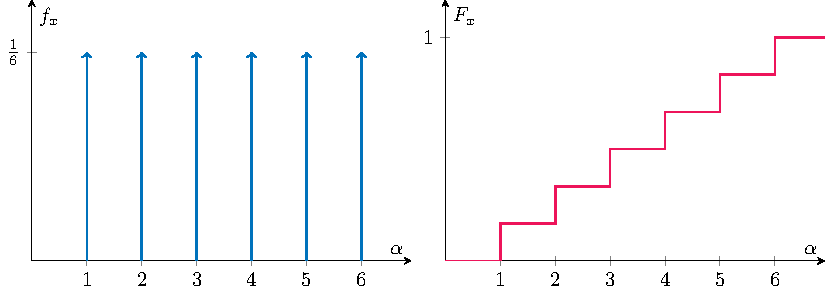
\includegraphics[width=0.9\columnwidth, page=1]{drwg_3.pdf}
\end{figure}
\subsection{Corrélation}
\begin{figure}[H]
\centering
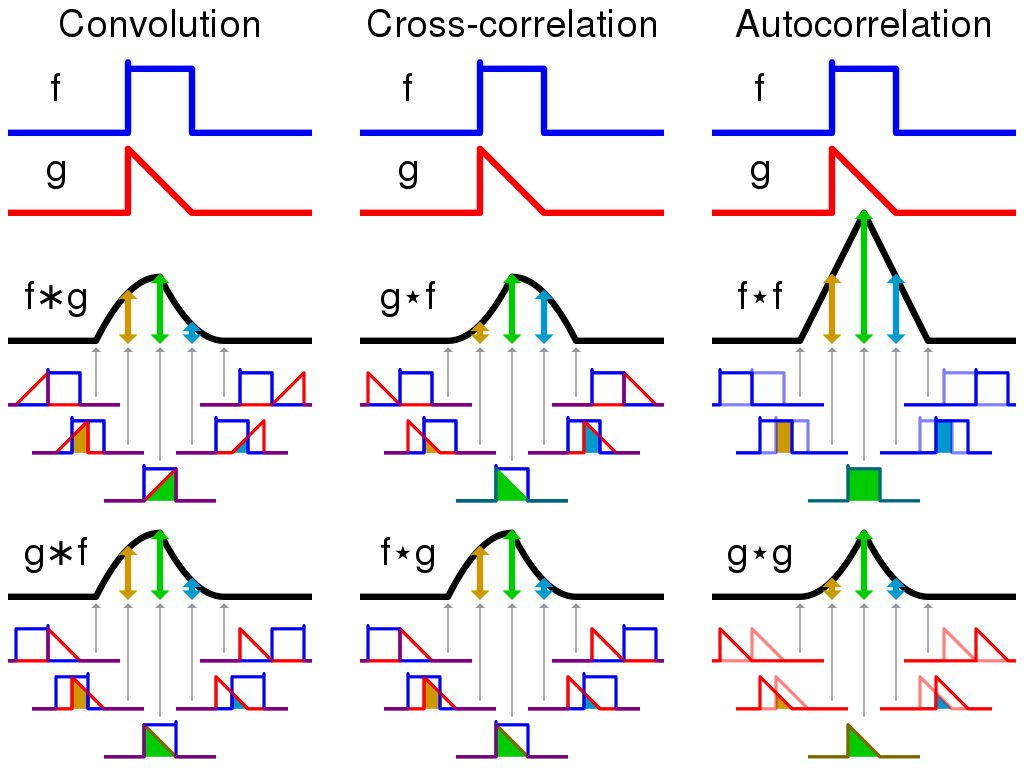
\includegraphics[width=\columnwidth]{img_3.png}
\end{figure}
$$r_{xy}(k,l)=E\lbrace x(k)y^\ast(l)\rbrace$$
Si $x$ et $y$ sont indépendants :
$$r_{xy}(k,l)=0$$
Avec ${}^\ast$ le conjugué complexe (si les valeurs sont complexes). Si la corrélation est le produit des moyennes, alors les deux variables sont indépendantes
$$r_{xy}=E\lbrace x\rbrace E\lbrace y^\ast\rbrace=m_xm_y^\ast\longrightarrow\text{ indépendants}$$
\subsection{Coefficient de corrélation}
$$\rho_{xy}=\frac{\text{cov}(x,y)}{\sigma_x\sigma_y}\leq 1$$
\subsection{Gaussienne}
$$f_x(\alpha)=\frac{1}{\sigma_x\sqrt{2\pi}}\text{exp}\left(-\frac{(\alpha-m_x)^2}{2\sigma_x^2}\right)$$
\begin{figure}[H]
\centering
\includegraphics[width=6cm ,page=3]{drwg_3.pdf}
\end{figure}
\subsection{Bruit blanc}
Avec déviation standard de $\sigma$
$$P=\sigma^2$$
Le spectre est plat entre $-\frac{F_s}{2}$ et $\frac{F_s}{2}$ avec une amplitude de $\sigma^2$


\end{document}